\begin{itemize}
	\item \textbf{Энтропийное кодирование}~\
	
	Как говорилось ранее, энтропия показывает наименьшее среднее число бит, необходимое для кодирования некоторой информации. Данное свойство используется, как ни странно, при кодировании информации.
	
	Например, код Шеннона-Фано. С целью минимизации энтропии и, соответственно, оптимизации кода элементы с большой вероятностью появления кодируются меньшим числом символом. Таким образом, производится сжатие объема информации, что позволяет передавать большее количество информации, затрачивая меньший объем памяти.
	
	\item \textbf{Построение решающих деревьев}
	
	Решающие деревья - метод, использующийся в машинном обучении и работающий по принципу принятия решений человеком. Каждое ветвление представляет собой разделение выборки на 2 части по порогу некоторого признака. Например, признак - длина, пороговое значение -  2,5. Все объекты, длина которых превышает 2,5, отделяются от объектов с длиной меньше 2,5 и дальнейший анализ проходят отдельно.
	
	В данном методе расчет энтропии помогает определить оптимальный порог для каждого узла решения. А именно, подбирается такое разделение выборки, при котором сумма энтропий получившихся выборок минимальна среди возможных вариантов разбиений.
	
	Это позволяет получать после разбиения выборки, наименее разнообразные по содержанию классов. Соответственно, признак и пороговое значение подбираются наиболее оптимально - алгоритм успешно отделяет объекты, принадлежащие одному классу.
	
	\item \textbf{Применение в алгоритмах t-SNE и UMAP}
	
	В анализе данных часто возникает необходимость в снижении размерности, и в таких случаях на помощь приходят знания об энтропии, изученной в курсе теории вероятностей. Речь, конечно, идет не об энтропии как таковой, а об алгоритмах, которые базируются на теории.
	
	При создании пространства меньшей размерности, t-SNE и UMAP используют кросс-энтропию как показатель эффективности перенесения свойств объектов. Чем меньше кросс-энтропия, тем ближе к истинному оказалось подобранное распределение.
	
	Приведем пример работы алгоритма UMAP. Мы возьмем набор данных об одежде, который включает в себя 70000 черно-белых изображений различной одежды по 10 классам: футболки, брюки, свитеры, платья, кроссовки и т.д. Каждая картинка имеет размер 28x28 пикселей или 784 пикселя всего (то есть изначально у нас имеется 784-мерное пространство). UMAP перевел его в 2-мерное и визуализировал результат (см. ниже).
	
	\begin{listing}[1]{1}
import numpy as np #импортируем библиотеку Numpy, чтобы работать с матрицами
from mnist import MNIST #импортируем библиотеку MNIST с наборами данных
#импортируем библиотеку matplotlib для построения графиков
import matplotlib.pyplot as plt
%matplotlib inline
		
mndata = MNIST('fashionmnist') #выбираем набор данных с фотографиями одежды
#обычно в машинном обучении выборку делят на обучающую и тестовую, чтобы
#обучить алгоритм и проверить, как он работает, но нам это не понадобится
#сохраняем обучающую выборку
#в переменную train сохраняется выборка с признаками объектов (фотографиями)
#в train_labels - ответы, то есть категории одежды,
#которые изображены на соответствующих фотографиях
train, train_labels = mndata.load_training() 
test, test_labels = mndata.load_testing() #сохраняем тестовую выборку
#соединяем обучающую и тестовую выборку с признаками
data = np.array(np.vstack([train, test]), dtype=np.float64) / 255.0
#соединяем обучающую и тестовую выборку с ответами
target = np.hstack([train_labels, test_labels])
#записываем список из наименований одежды
classes = [
	'T-shirt/top',
	'Trouser',
	'Pullover',
	'Dress',
	'Coat',
	'Sandal',
	'Shirt',
	'Sneaker',
	'Bag',
	'Ankle boot']
			
import umap #импортируем библиотеку с алгоритмом UMAP

#анализируем набор данных
embedding = umap.UMAP(n_neighbors=10).fit_transform(data)
		
#рисуем график из получившегося нового распределения данных embedding
fig, ax = plt.subplots(1, figsize=(14, 10))
plt.scatter(*embedding.T, s=0.5, c=target, cmap='Spectral', alpha=1.0)
cbar = plt.colorbar(boundaries=np.arange(11)-0.5)
plt.setp(ax, xticks=[], yticks=[])
cbar.set_ticks(np.arange(10))
cbar.set_ticklabels(classes)
plt.title('Fashion MNIST Embedded via UMAP')
	\end{listing}

Вот что вышло:

\begin{figure}[bh]
	\noindent\centering{
		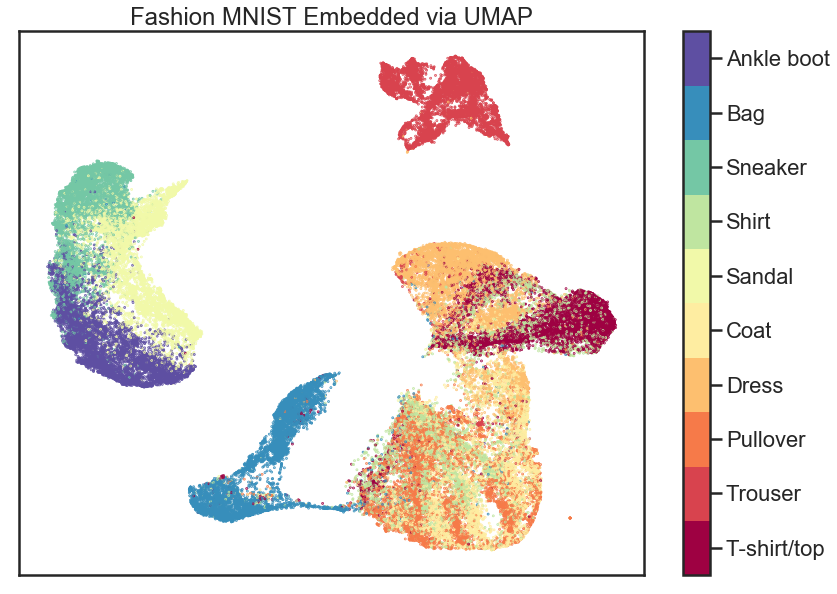
\includegraphics[height=70mm, width=110mm]{umap.png}
	}
	\caption{Алгоритм UMAP}
	\label{figCurves}
\end{figure}

Изначально каждый пиксель являлся признаком объекта (фотографии) и принимал некоторое значение (цвет). Если бы каждая картинка состояла из 2 пикселей, мы бы смогли построить график, где по оси абсцисс отложен цвет 1 пикселя, по оси ординакт цвет 2 пикселя и изобразить точками все объекты.

В нашем случае из-за большого количества пикселей мы не можем так сделать с исходной выборкой. Однако, если мы преобразуем выборку таким образом, что останется всего лишь 2 признака, то мы сможем визуализировать и ее. Только получившиеся 2 признака будут уже не пикселями, а абстрактными признаками, которые алгоритм получает из исходных.

Но получить такие 2 абстрактных признака можно очень многими способами. Но при этом нам необходимо, чтобы получившиеся 2 признака описывали исходную выборку как можно лучше - чтобы при визуализации мы видели не случайно нарисованное изображение, а некоторое отображение начального пространства. Именно тут алгоритм применяет кросс-энтропию. Минимизируя кросс-энтропию, между двумя распределениями (истинным и созданным алгоритмом), мы сокращаем отличия между ними, что позволяет получить максимально приближенный к нужному результат.
\end{itemize}